\section{Making a New RAVEN Plugin}

Creating a new plugin is a straightforward process. It involves setting up a repository,
establishing a basic structure, and installing in RAVEN for testing.

%\subsection{Setting up a Repository}
%TODO

\subsection{Plugin Structure}
The following directories must be present in the main directory of the plugin in order for RAVEN to
read it correctly:
\begin{itemize}
  \item \texttt{src}, where the entities for RAVEN to load are located;
  \item \texttt{doc}, where the documentation for the plugin and its entities is located.
  \item \texttt{tests}, where continuous integration tests are located;
\end{itemize}

\subsection{Additional Libraries}
If the plugin requires additional libraries, they can extend the \texttt{dependencies.xml} file in
the same manner as RAVEN's dependencies file. Libraries will be added like they are for RAVEN
itself, and a check will be performed to assure no base RAVEN (or other plugin) dependencies are
modified.

\subsection{Installing in RAVEN}
Use the installation script in \texttt{raven/scripts/install\_plugins.py}.
\begin{lstlisting}[morekeywords={examplePlugin, pluginInstallation}]
  raven/scripts/install_plugins.py -s /abs/path/to/pluginName
\end{lstlisting}
Replacing \texttt{pluginName} with the path to your plugin and the name of the directory, such as
\texttt{/user/projects/raven/plugins/pluginName}.
Use the absolute path to your new plugin to avoid any navigation problems.
If installing an officially-supported plugin that you do not plan on modifying, the following command
can be run (using TEAL as the example plugin):
\begin{lstlisting}[morekeywords={examplePlugin, TEALInstallation}]
  raven/scripts/install_plugins.py -s TEAL
\end{lstlisting}
Note the path was eliminated. This will initialize (or update) the official plugin in
\texttt{raven/plugins} with the official submoduled version.
To install all officially-supported plugins, the shortcut option \texttt{-a} or \texttt{--all} can be used:
\begin{lstlisting}[morekeywords={examplePlugin, installAllPlugin}]
  raven/scripts/install_plugins.py -a
\end{lstlisting}
At this stage, RAVEN will import all the plugins within that directory and perform some error checking.

This process automatically registers the plugin in the plugin directory, and informs the plugin
about RAVEN %(TODO more notes on this!)

\subsection{Using the Plugin in RAVEN}
Once registered/installed, the new entity (i.e., ExternalModel, ROM, PostProcessor) can be used in RAVEN by
using the entity subtype defined by your plugin name. For example, if your external model class is named "myPluginModel",
you can access an external model in the RAVEN input as

\begin{lstlisting}[morekeywords={usingPlugin}]
<Models>
  ...
  <ExternalModel name='myName' subType='pluginName.myPluginModel'>
    ...
  </ExternalModel>
  ...
</Models>
\end{lstlisting}

\subsection{Adding Testers}
RAVEN automatically provides a testing harness for automated regression testing. This includes a
variety of \emph{testers}, such as CSV checkers and XML checkers.

If a plugin requires additional testers for regression testing, they can be added to the plugin and
loaded by RAVEN's test harness at testing time.

Any new testers should be added under a folder named \texttt{Testers} in the \texttt{src} directory
of the plugin. For example, for a plugin named \texttt{examplePlugin} and a tester named
\texttt{myNewTester}:
\begin{lstlisting}[morekeywords={examplePlugin,myNewTester}]
  /path/to/examplePlugin/src/Testers/myNewTester.py
\end{lstlisting}
Any discovered testers will be made available to the \texttt{tests} files used by the RAVEN
regression test system; for example:
\begin{lstlisting}[morekeywords={myNewTester}]
[Tests]
  [./aTestForMyPlugin]
    type = myNewTester
    input = my_test_input.xml
    csv = 'TestWorkingDir/results.csv'
  [../]
[]
\end{lstlisting}

For more information on inheriting from and creating new testers, see the RAVEN regression system
documentation.

\subsection{Adding A New Plugin}
\begin{figure}
\centering
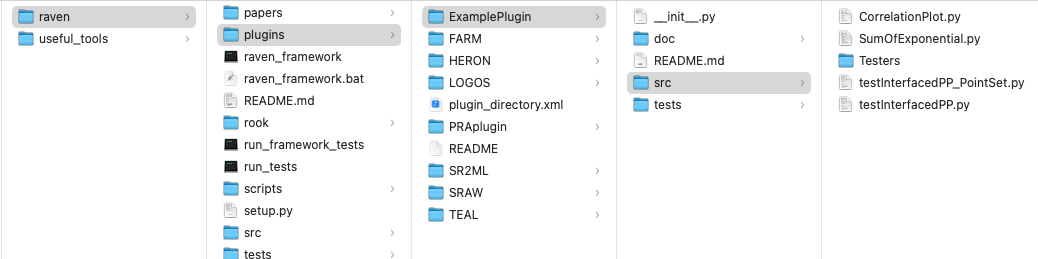
\includegraphics[width=1.0\textwidth]{pics/plugins_location.png}
\caption{Plugins Location}
\label{fig:pluginsLocation}
\end{figure}
The procedure of adding a plugin for RAVEN is a straightforward process.
The addition of a plugin does not require modifying RAVEN itself.
Instead, the developer creates a new Python module that is going to be embedded
in RAVEN at run-time (no need to introduce  hard-coded statements), if this Python module
inherits from one of the following RAVEN plugin base classes located at \texttt{raven/ravenframework/PluginBaseClasses}:
\begin{lstlisting}[language=bash]
 ExternalModelPluginBase in ExternalModelPluginBase.py
 PlotPlugin in OutStreamPlotPlugin.py
 PostProcessorPluginBase in PostProcessorPluginBase.py
 SupervisedLearningPlugin in SupervisedLearningPlugin.py
\end{lstlisting}
These classes can be loaded as follows:
\begin{lstlisting}[language=bash]
 from ravenframework.PluginBaseClasses.ExternalModelPluginBase import ExternalModelPluginBase
 from ravenframework.PluginBaseClasses.OutStreamPlotPlugin import OutStreamPlotPlugin
 from ravenframework.PluginBaseClasses.PostProcessorPluginBase import PostProcessorPluginBase
 from ravenframework.PluginBaseClasses.SupervisedLearningPlugin import PlotPlugin
\end{lstlisting}
The APIs for these classes can be either found in the following sections or directly in the modules themselves.

If the plugin developer wants to make of his plugin
an official supported plugin in RAVEN (by the submodule system), he needs to check
the raven wiki under the ``contribution'' section), and this plugin needs to be placed in a folder (whatever name) located
in (see figure~\ref{fig:pluginsLocation}):
\begin{lstlisting}[language=bash]
 path/to/raven/plugins/
\end{lstlisting}
